\chapter{Something to Protect: Hermione Granger}

\lettrinepara{A}{nd} it was evening and it was morning, the last day. June 15th, 1992.

\hplettrineextrapara
The beginning light of morning, the pre-dawn before sunrise, was barely brightening the sky. To the east of Hogwarts, where the Sun would rise, that faintest tinge of grey made barely visible the hilly horizon beyond the Quidditch stands.

The stone terrace-platform where Harry now sat would be high enough to see the dawn beyond the hills below; he’d asked for that, when he was describing his new office.

Harry was currently sitting cross-legged on a cushion, chilly pre-morning breezes stirring over his exposed hands and face. He’d ordered the house elves to bring up the hand-glittered throne from his previous office as General Chaos…and then he’d told the elves to put it back, once it had occurred to Harry to start worrying about where his taste in decorations had come from and whether Voldemort had once possessed a similar throne. Which, itself, wasn’t a knockdown argument—it wasn’t like sitting on a glittery throne to survey the lands below Hogwarts was \emph{unethical} in any way Harry’s moral philosophy could make out—but Harry had decided that he needed to take time and think it through. Meanwhile, simple cushions would do well enough.

In the room below, connected to the rooftop by a simple wooden ladder, was Harry’s new office inside Hogwarts. A wide room, surrounded by full-wall windows on four sides for sunlight; currently bare of furnishings but for four chairs and a desk. Harry had told Headmistress McGonagall what he was looking for, and Headmistress McGonagall had put on the Sorting Hat and then told Harry the series of twists and turns that would take him where he wanted to be. High enough in Hogwarts that the castle shouldn’t have been that tall, high enough in Hogwarts that nobody looking from the outside would see a piece of castle corresponding to where Harry now sat. It seemed like an elementary precaution against snipers that there was no reason \emph{not} to take.

Though, on the flip side, Harry had no idea where he currently \emph{was} in any real sense. If his office couldn’t be seen from the lands below, then how was Harry seeing the lands, how were photons making it from the landscape to him? On the western side of the horizon, stars still glittered, clear in the pre-dawn air. Were those photons the actual photons that had been emitted by huge plasma furnaces in the unimaginable distance? Or did Harry now sit within some dreaming vision of the Hogwarts castle? Or was it all, without any further explanation, ‘just magic’? He needed to get electricity to work better around magic so he could experiment with shining lasers downward and upward.

And yes, Harry had his own office on Hogwarts now. He didn’t have any official title yet, but the Boy-Who-Lived was now a true fixture of the Hogwarts School of Witchcraft and Wizardry, the soon-to-be-home of the Philosopher’s Stone and the world’s only wizarding institution of genuinely higher education. It wasn’t fully secured, but Professor Vector had put up some preliminary Charms and Runes to screen the office and its rooftop against eavesdropping.

Harry sat on his cushion, near the edge of his office’s roof, and gazed down upon trees and lakes and flowering grass. Far below, carriages sat motionlessly, not yet harnessed to skeletal horses. Small boats littered the shore, prepared to ferry younger students across the lake when the time came. The Hogwarts Express had arrived overnight, and now the carriages and the huge old-fashioned engine awaited on the other side of the southern lake. All was ready to take the students home after the Leave-Taking Feast in the morning.

Harry stared across the lake, at the great old-fashioned locomotive he wouldn’t be riding home this time. Again. There was a strange sadness and worry to that thought, like Harry was already starting to miss out on the bonding experiences with \emph{the other students his age}—if you could say that at all, when a significant part of Harry had been born in 1926. It had felt to Harry, last night in the Ravenclaw common room, like the gap between him and the other students had, yes, widened even further. Though that might only have been from the questions Padma Patil and Anthony Goldstein had excitedly asked each other about the Girl-Who-Revived, the rapid-fire speculations shooting through the air from Ravenclaw to Ravenclaw. Harry had known the answers, he’d known all the answers, and he hadn’t been able to say them.

There was a part of Harry that was tempted to go on the Hogwarts Express and then come back to Hogwarts by Floo. But when Harry imagined finding five other students for his compartment, and then spending the next eight hours keeping secrets from Neville or Padma or Dean or Tracey or Lavender…it didn’t seem like an attractive prospect. Harry felt like he ought to do it for reasons of Socializing with the Other Children, but he did not \emph{want} to do it. He could meet with everyone again at the start of the next school year, when there would be other topics of which he could speak more freely.

Harry stared south across the lake, at the huge old locomotive, and thought about the rest of his life.

About the Future.

The prophecy Dumbledore’s letter had mentioned about him tearing apart the stars in heaven…well, \emph{that} sounded optimistic. That part had an obvious interpretation to anyone who’d grown up with the right sort of upbringing. It described a future where humanity had won, more or less. It wasn’t what Harry usually thought about when he gazed at the stars, but from a truly \emph{adult} perspective, the stars were enormous heaps of valuable raw materials that had unfortunately caught fire and needed to be scattered and put out. If you were tapping the huge hydrogen-helium reservoirs for raw materials, that meant your species had successfully grown up.

Unless the prophecy had been referring to something else entirely. Dumbledore might have been misinterpreting some seer’s words…but his message to Harry had been phrased as if there’d been a prophecy about Harry \emph{personally} tearing apart stars, in the foreseeable future. Which seemed potentially more worrisome, though by no means certain to be true, or a bad thing if it was true…

Harry vented a sigh. He’d begun to understand, in the long hours before sleep had taken him last night, just what Dumbledore’s last message implied.

Looking back on the events of the 1991–1992 Hogwarts school year was nothing short of bone-freezingly terrifying, now that Harry understood what he was seeing.

It wasn’t just that Harry had kept the frequent company of his good friend Lord Voldemort. It wasn’t even \emph{mostly} that.

It was the vision of a narrow line of Time that Albus Dumbledore had steered through fate’s narrow keyhole, a hair-thin strand of possibility threaded through a needle’s eye.

The prophecies had instructed Dumbledore to have Tom Riddle’s intelligence copied onto the brain of a wizarding infant who would then grow up learning Muggle science. What did it say about the likely shape of the Future, if \emph{that} was the first or best strategy the seers could find that \emph{didn’t} lead to catastrophe?

Harry could look back now on the Unbreakable Vow that he’d made, and guess that if not for that Vow, disaster might have already been set in motion yesterday when Harry had wanted to tear down the International Statute of Secrecy. Which in turn strongly suggested that the many prophecies Dumbledore had read and whose instructions he’d followed, had somehow ensured that Harry and Voldemort would collide in \emph{exactly the right} way to cause Voldemort to force Harry to make that Unbreakable Vow. That the Unbreakable Vow had been part of Time’s narrow keyhole, one of the improbable preconditions for allowing the Earth’s peoples to survive.

A Vow whose sole purpose was to protect everyone from Harry’s current \emph{stupidity}.

It was like watching a videotape of an almost-traffic-accident that had happened to you, where you remembered another car missing you by centimetres, and the video showing that somebody had \emph{also} thrown a pebble in exactly the right way to cause an enormous lorry to miss that near-collision, and if they hadn’t thrown that pebble then you and all your family in the car and your \emph{entire planet} would have been hit by the lorry, which, in the metaphor, represented your own \emph{sheer obliviousness.}

Harry had been \emph{warned}, he’d \emph{known} on some level or the Vow wouldn’t have stopped him, and yet he’d \emph{still} almost made the wrong choice and destroyed the world. Harry could look back now and see that, yes, the alternate Harry with no Vow would’ve had trouble accepting the reasoning that said you couldn’t get magical healing to Muggles as fast as possible. If the alternate Harry had acknowledged the danger at all, he would have rationalized it, tried to figure out some clever way around the problem and refused to accept \emph{taking a few years longer to do it,} and so the world would have ended. Even after all the warnings Harry had received, it \emph{still} wouldn’t have worked without the Unbreakable Vow.

One tiny strand of Time, being threaded through a needle’s eye.

Harry didn’t know how to handle this revelation. It wasn’t a sort of situation that human beings had evolved emotions to handle. All Harry could do was stare at how close he had come to disaster, might come \emph{again} to disaster if that Vow was fated to trigger more than once, and think…

Think…

‘I don’t want that to happen again’ didn’t seem like the right thought. He’d never \emph{wanted} to destroy the world in the first place. Harry hadn’t lacked for protective feelings about Earth’s sapient population, those protective feelings had been the \emph{problem} in a way. What Harry had lacked was some element of clear vision, of being willing to consciously acknowledge what he’d already known deep down.

And the whole thing with Harry having spent the last year cosying up to the Defence Professor didn’t speak highly of his intellect either. It seemed to point to the same problem, even. There were things Harry had known or strongly suspected on some level, but never promoted to conscious attention. And so he had failed and nearly died.

\emph{I need to raise the level of my game.}

That was the thought Harry was looking for. He had to do better than this, become a less stupid person than this.

\emph{I need to raise the level of my game, or fail.}

Dumbledore had destroyed the recordings in the Hall of Prophecy and arranged for no further recordings to be made. There’d apparently been a prophecy that said Harry mustn’t look upon those prophecies. And the obvious next thought, which might or might not be true, was that saving the world was \emph{beyond the reach of prophetic instruction}. That winning would take plans that were too complex for seers’ messages, or that Divination couldn’t see somehow. If there’d been some way for Dumbledore to save the world himself, then prophecy would probably have told Dumbledore how to do that. Instead the prophecies had told Dumbledore how to create the preconditions for a particular sort of person existing; a person, maybe, who could unravel a challenge more difficult than prophecy could solve directly. That was why Harry had been placed on his own, to think without prophetic guidance. If all Harry did was follow mysterious orders from prophecies, then he wouldn’t mature into a person who could perform that unknown task.

And right now, Harry James Potter-Evans-Verres was still a walking catastrophe who’d needed to be constrained by an Unbreakable Vow to prevent him from \emph{immediately} setting the Earth on an inevitable course toward destruction \emph{when he’d already been warned against it.} That had happened \emph{literally yesterday,} just one day after he’d helped Voldemort almost take over the planet.

A certain line from Tolkien kept running through Harry’s mind, the part where Frodo upon Mount Doom put on the ring, and Sauron suddenly realized what a \emph{complete idiot} he’d been. ‘And the magnitude of his own folly was at last laid bare’, or however that had gone.

There was a huge gap between who Harry needed to become, and who he was right now.

And Harry didn’t think that time, life experience, and puberty would take care of that automatically, though they might help. Though if Harry could grow into an adult that was to \emph{this} self what a normal adult was to a normal eleven-year-old, maybe \emph{that} would be enough to steer through Time’s narrow keyhole…

He had to grow up, somehow, and there was no traditional path laid out before him for accomplishing that.

The thought came then to Harry of another work of fiction, more obscure than Tolkien:

\emph{You can only arrive at mastery by practising the techniques you have learned, facing challenges and apprehending them, using to the fullest the tools you have been taught, until they shatter in your hands and you are left in the midst of wreckage absolute…I cannot create masters. I have never known how to create masters. Go, then, and fail…You have been shaped into something that may emerge from the wreckage, determined to remake your Art. I cannot create masters, but if you had not been taught, your chances would be less. The higher road begins after the Art seems to fail you; though the reality will be that it was you who failed your Art.}

It wasn’t that Harry had gone down the \emph{wrong} path, it wasn’t that the road to sanity lay somewhere outside of science. But reading science papers hadn’t been \emph{enough}. All the cognitive psychology papers about known bugs in the human brain and so on had \emph{helped}, but they hadn’t been \emph{sufficient}. He’d failed to reach what Harry was starting to realise was a \emph{shockingly} high standard of being so incredibly, unbelievably rational that you actually started to \emph{get things right,} as opposed to having a handy language in which to describe afterwards everything you’d just done wrong. Harry could look back now and apply ideas like ‘motivated cognition’ to see where he’d gone astray over the last year. That counted for something, when it came to being saner in the future. That was better than having no idea what he’d done wrong. But that wasn’t yet being the person who could pass through Time’s narrow keyhole, the adult form whose \emph{possibility} Dumbledore had been instructed by seers to create.

\emph{I need to think faster, grow up faster…How alone am I, how alone will I be? Am I making the same mistake I made during Professor Quirrell’s first battle, when I didn’t realise Hermione had captains? The mistake I made when I didn’t tell Dumbledore about the sense of doom, once I realised Dumbledore probably wasn’t mad or evil?}

It would help if Muggles had classes for this sort of thing, but they didn’t. Maybe Harry could recruit Daniel Kahneman, fake his death, rejuvenate him with the Stone, and put him in charge of inventing better training methods…

Harry took the Elder Wand out of his robes, gazed again at the dark-grey wood that Dumbledore had passed down to him. Harry had \emph{tried} to think faster this time, he’d tried to complete the pattern implied by the Cloak of Invisibility and the Resurrection Stone. The Cloak of Invisibility had possessed the legendary power of hiding the wearer, and the hidden power of allowing the wearer to hide from Death itself in the form of Dementors. The Resurrection Stone had the legendary power of summoning an image of the dead, and then Voldemort had incorporated it into his horcrux system to allow his spirit to move freely. The second Deathly Hallow was a potential component of a system of true immortality that Cadmus Peverell had never completed, maybe due to his having ethics.

And then there was the third Deathly Hallow, the Elder Wand of Antioch Peverell, that legend said passed from wizard to stronger wizard, and made its holder invincible against ordinary attacks; that was the known and overt characteristic…

The Elder Wand that had belonged to Dumbledore, who’d been trying to prevent the Death of the world itself.

The purpose of the Elder Wand always going to the victor might be to find the strongest living wizard and empower them still further, in case there was any threat to their entire species; it could secretly be a tool to defeat Death in its form as the destroyer of worlds.

But if there was some higher power locked within the Elder Wand, it had not presented itself to Harry based on that guess. Harry had raised up the Elder Wand and spoken to it, named himself a descendant of Peverell who accepted his family’s quest; he’d promised the Elder Wand that he would do his best to save the world from Death, and take up Dumbledore’s duty. And the Elder Wand had answered no more strongly to his hand than before, refusing his attempt to jump ahead in the story. Maybe Harry needed to strike his first true blow against the Death of worlds before the Elder Wand would acknowledge him; as the heir of Ignotus Peverell had already defeated Death’s shadow, and the heir of Cadmus Peverell had already survived the Death of his body, when their respective Deathly Hallows had revealed their secrets.

At least Harry had managed to guess that, contrary to legend, the Elder Wand didn’t contain a core of ‘Thestral hair’. Harry had seen Thestrals, and they were skeletal horses with smooth skin and no visible mane on their skull-like heads, nor tufts on their bony tails. But what core was truly inside the Elder Wand, Harry hadn’t yet felt himself knowing; nor had he been able to find, anywhere on the Elder Wand, the circle-triangle-line of the Deathly Hallows that should have been present.

“I don’t suppose,” Harry murmured to the Elder Wand, “you could just tell me?”

There came back no answer from the globe-knobbed wand; only a sense of glory and contained power, watching him skeptically.

Harry sighed, and put the most powerful wand in the world back into his school robes. He’d get it eventually, and hopefully in time.

Maybe faster, if there was someone to help him do the research.

Harry was aware on some level—no, he needed to stop being aware of things \emph{on some level} and start just being aware of them—Harry was explicitly and consciously aware that he was ruminating about the Future mostly to distract himself from the imminent arrival of Hermione Granger. Who would receive a clear bill of health from St. Mungo’s, when she woke up very early this morning, and who would then Floo with Professor Flitwick back to Hogwarts. Whereupon she’d tell Professor Flitwick that she needed to speak with Harry Potter immediately. There’d been a note from Harry to himself about that, when Harry had woken up later this morning with the sun already risen in the Ravenclaw dorm. He’d read the note, and then Time-Turned back to before the dawn hour when Hermione Granger would arrive.

\emph{She won’t actually be angry with me.}

…

\emph{Seriously. Hermione isn’t that kind of person. Maybe she was at the start of the year but she’s too self-aware to fall for that one now.}

…

\emph{What do you mean, ‘…’? If you have something to say, inner voice, just say it! We’re trying to be more aware of our own thought processes, remember?}

\later

The sky had gone full blue-grey, dawn barely short of sunrise, by the time that Harry heard the sound of footsteps coming from the ladder that opened into his new office. Hastily Harry stood up and began to brush off his robes; and then, realising what he was doing, stopped the nervous motions. He’d just defeated Voldemort, damn it, he ought not to be this nervous.

The young witch’s head and chestnut curls appeared in the opening and peered around. Then she rose up higher, seemed almost to run up the ladder steps, like she was walking along an ordinary pavement but vertically; Harry could have blinked and missed it, how her shoe came down on the top rung of the ladder and then she leaped lightly onto the roof an instant later.

\emph{Hermione.} Harry’s lips moved around the word, but made no sound.

There’d been something Harry had meant to say, but it had gone right out of his mind.

Maybe a quarter of the minute passed, on the rooftop, before Hermione Granger spoke. She was wearing a blue-edged uniform now, and the blue-bronze-striped tie of her proper House.

“Harry,” said Hermione Granger, a terribly familiar voice that almost brought tears to Harry’s eyes, “before I ask you all the questions, I’d like to start by saying thank you very much for, um, whatever it is you did. I mean it, really. Thank you.”

“Hermione,” Harry said, and swallowed. The phrase \emph{may I have permission to hug you,} which Harry had imagined using for his opening line, seemed impossible to say. “Welcome back. Hold on while I put up some privacy spells.” Harry took the Elder Wand out of his robes, got a book from his pouch that he opened to a bookmark, and then carefully pronounced “\emph{Hominem Revelio,}” along with two other recently-acquired security Charms that Harry had found himself barely able to cast if he wielded the Elder Wand. It wasn’t much, but it was marginally better security than just relying on Professor Vector.

“You have Dumbledore’s wand,” Hermione said. Her voice was hushed, and sounded as loud as an avalanche in the still dawn air. “And you can use it to cast fourth-year spells?”

Harry nodded, making a mental note to be more careful who else saw him do that. “Is it okay if I hug you?”

Hermione moved lightly over to him; her movements were peculiarly swift, more graceful than they’d been before. Her motions seemed to radiate an air of something pure and untouched, reminding Harry again of how peaceful Hermione had looked when she was sleeping on Voldemort’s altar—

Realization hit Harry like a ton of bricks, or at least a kilogram of brick.

And Harry hugged Hermione, feeling how very \emph{alive} she seemed. He felt like crying, and suppressed it, because he didn’t know whether that was just her aura affecting him or not.

Hermione’s arms around him were gentle, exceedingly light in their pressure, as if she were being deliberately careful not to snap his body in half like a used toothpick.

“So,” Hermione said, once Harry had let go of her. Her young face looked very serious, as well as pure and innocent. “I didn’t tell the Aurors you were there, or that it was Professor Quirrell and not You-Know-Who who killed all the Death Eaters. Professor Flitwick only let them give me one drop of Veritaserum, so I didn’t have to say. I just told them the troll was the last thing I remembered.”

“Ah,” Harry said. He had somehow found himself staring at Hermione’s nose instead of her eyes. “What do you think happened, exactly?”

“Well,” Hermione Granger said thoughtfully, “I got eaten by a troll, which I’d frankly rather not do again, and then there was a really loud \emph{bang} and my legs were back, and I was lying on a stone altar in the middle of a graveyard in a dark moonlit forest I’d never seen before, with somebody’s severed hands clutched around my throat. So you see, Mr~Potter, finding myself in a situation that weird and dark and scary, I wasn’t going to make the same mistake I did last time with Tracey. I knew \emph{right away} that it was you.”

Harry nodded. “Good call.”

“I said your name, but you didn’t answer,” said Hermione. “I sat up and one of the bloody hands slid down over my shirt, leaving little bits of flesh behind. I didn’t scream though, even when I looked around and saw all the heads and bodies and realized what the smell was.” Hermione stopped, took another deep breath. “I saw the skull masks and realized that the dead people had been Death Eaters. I knew right away that the Defence Professor had been there with you and killed them all, but I didn’t notice Professor Quirrell’s body was also there. I didn’t realize it was him even when I saw Professor Flitwick checking the body. He looked…different, when he was dead.” Hermione’s voice became quieter. She looked humbled somehow, in a way Harry couldn’t often remember seeing. “They said David Monroe sacrificed his life to bring me back, the same way your mother sacrificed herself for you, so that the Dark Lord would explode again when he tried to touch me. I’m \emph{pretty} sure that’s not the whole truth, but…I’ve thought a lot of nasty things about our Defence Professor that I never should’ve thought.”

“Um,” Harry said.

Hermione nodded solemnly, her hands clasped in front of her as though in penitence. “I know you’re probably too nice to say the things to me that you have a right to say now, so I’ll say them for you, Harry. You were right about Professor Quirrell, and I was wrong. You told me so. David Monroe was a little bit Dark and a whole lot Slytherin, and it was childish of me to think that was the same thing as being evil.”

“Ah…” Harry said. This was very hard to say. “Actually, the rest of the world doesn’t know this part, not even the Headmistress. But in point of fact you were one hundred and twelve percent correct about him being evil, and I’ll remember for future reference that although ‘Dark’ and ‘evil’ may not technically be the same thing, there’s a great big statistical correlation.”

“Oh,” said Hermione, and fell silent again.

“You’re not saying that you told me so?” said Harry. His mental model of Hermione was yelling: \shout{I told you so! Didn’t I tell you so, Mr~Potter? Didn’t I tell you? Professor Quirrell is eeeeviiil, I said, but \emph{you didn’t listen to me!}}

The actual Hermione just shook her head. “I know you cared about him a lot,” she said softly. “Since I was right after all…I knew you’d probably be hurting a lot after Professor Quirrell turned out to be evil, and that it wouldn’t be a good time to say I told you so. I mean, that’s what I decided when I was thinking that part through several months earlier.”

\emph{Thank you, Miss~Granger.} Harry was glad she’d said that much, though, it just wouldn’t have felt like Hermione otherwise.

“So, Mr~Potter,” said Hermione Granger, tapping her fingers on her robe at around thigh level. “After the medi-witch drew my blood, it stopped hurting right away, and when I brushed away the little bit of blood on my arm, I couldn’t find where the needle had poked me. I bent some of the metal in my bed frame without trying hard, and though I haven’t had a chance to test it yet, I feel like I should be able to run really \emph{fast}. My fingernails are pearly white and shiny even though I don’t remember painting them. And my teeth look like that too, which, being the daughter of dentists, makes me nervous. So it’s not that I’m ungrateful, but just what exactly did you do?”

“Um,” Harry said. “And I’m expecting you’re also wondering why you’re radiating an aura of purity and innocence?”

“I’m \emph{what?}”

“That part wasn’t my idea. Honestly.” Harry’s voice went small. “Please don’t kill me.”

Hermione Granger raised her hands in front of her face, staring somewhat cross-eyed at her fingers. “Harry, are you saying…I mean, my radiating innocence and being all fast and graceful and my teeth being pearly white…is it \emph{alicorn} my fingernails are made of?”

“Alicorn?”

“It’s the term for unicorn horn, Mr~Potter.” Hermione Granger seemed to be trying to nibble her fingernails, and not having much luck. “So, I guess if you bring a girl back from the dead she ends up as, what did Daphne call it, a Sparkling Unicorn Princess?”

“That’s not exactly what happened,” Harry said, though it was frighteningly close.

Hermione took her finger out of her mouth, frowning at it. “I can’t bite through it either. Mr~Potter, did you consider the problems now that it’s literally impossible for me to trim my fingernails and toenails?”

“The Weasley twins have a magical sword that should work,” Harry volunteered.

“I think,” Hermione Granger said firmly, “that I would like to know the whole story behind all this, Mr~Potter. Because knowing you and knowing Professor Quirrell, there was some sort of \emph{plan} going on.”

Harry took a deep breath. Then he exhaled. “Sorry, it’s…classified. I could tell you if you studied Occlumency, but…do you want to?”

“Do I want to study Occlumency?” Hermione said, looking slightly surprised. “That’s at least a sixth-year thing, isn’t it?”

“I learned it,” Harry said. “I started with an unusual boost, but I doubt that really mattered in the long run. I mean, I’m sure you could learn calculus if you studied hard, regardless of what age Muggles usually learn it. The question is, um.” Harry was having to control his breathing. “The question is, do you still want to do…that kind of stuff.”

Hermione turned, and looked at where the sky was lightening in the east. “You mean,” she said quietly, “do I still want to be a hero now that it’s earned me a horrible death that one time.”

Harry nodded, then said “Yes” because Hermione wasn’t turning toward him, though the word felt blocked in his throat.

“I’ve been thinking about that,” Hermione said. “It was, in fact, an exceptionally gruesome and painful death.”

“I, um. I did set some things up \emph{just in case} you still wanted to be a hero. There were some short windows of opportunity where I didn’t have time to consult you, I couldn’t let you see me because I expected you to be given Veritaserum later. But if you don’t like it, I can undo most of what I did and you can just ignore the rest.”

Hermione nodded distantly. “Like making everyone think that I…Harry, \emph{did} I actually do anything to You-Know-Who?”

“No, that was all me, though please don’t tell anyone that. Just so you know, that time the Boy-Who-Lived supposedly defeated Voldemort, on the night of Halloween in 1981, that was Dumbledore’s victory and he let everyone think it was me. So now I’ve defeated a Dark Lord once, and had the credit for it once. It all balances out eventually, I guess.”

Hermione went on gazing to the east. “I’m not really comfortable with this,” she said after a while. “People thinking I defeated the Dark Lord Voldemort, when I haven’t done anything at all…oh, that’s the same thing you went through, isn’t it?”

“Yeah. Sorry about inflicting that on you. I was…well, I was trying to create a separate identity for you in people’s minds, I guess. There was just the one opportunity and everything was sort of \emph{rushed} and…I realized afterwards that maybe I shouldn’t have, but it was too late.” Harry cleared his throat. “Though, um. If you’re feeling like you want to do something that’s actually worthy of the way people think about the Girl-Who-Revived, um. I might have an idea for what you can do. Very soon, if you want.”

Hermione Granger was giving him a \emph{look}.

“But you don’t \emph{have} to!” Harry said hastily. “You can just ignore this whole thing and be the best student in Ravenclaw! If that’s what you prefer.”

“Are you trying to use reverse psychology on me, Mr~Potter?”

“No! Honestly!” Harry took a deep breath. “I’m \emph{trying} not to decide your life for you. I thought I saw, yesterday, I thought I saw what might come next for you—but then I remembered how much of this year I’d spent being a total idiot. I thought of some things Dumbledore said to me. I realized it genuinely wasn’t my place to say. That you could do anything you wanted with your life, and that above all, the choice had to be your own. Maybe you \emph{don’t} want to be a hero after this, maybe you want to become a great magical researcher because that’s who Hermione Granger really was all along, never mind what your fingernails are made out of now. Or you could go to the Salem Witches’ Institute in America instead of Hogwarts. I won’t lie and say I’d like that, but it really is up to you.” Harry turned to the horizon and swept his hand wide, as though to indicate all the world that lay beyond Hogwarts. “You can go \emph{anywhere} from here. You can do \emph{anything} with your life. If you want to be a wealthy sixty-year-old merman, I can make it happen. I’m serious.”

Hermione nodded slowly. “I’m curious about how you’d do that exactly, but what I want isn’t to have things done \emph{for} me.”

Harry sighed. “I understand. Um…” Harry hesitated. “I think…if it helps you to know…in my case, things were being arranged for me a \emph{lot}. By Dumbledore, mostly, though Professor Quirrell too. Maybe the power to earn your own way in life is itself something you have to earn.”

“Why, that sounds very wise,” Hermione said. “Like my parents paying for me to go to university, so I can some day get my own job. Professor Quirrell bringing me back to life as a Sparkling Unicorn Princess and you telling everyone that I offed the Dark Lord Voldemort is just like that, really.”

“I \emph{am} sorry,” Harry said. “I know I should’ve done it differently, but…I didn’t have much time to plan and I was exhausted and not really thinking straight—”

“I’m grateful, Harry,” Hermione said, her voice softer now. “You’re being too harsh on yourself, even. Please don’t take it so seriously when I’m sarcastic to you. I don’t want to be the sort of girl who comes back from the dead, and then starts complaining about which superpowers she got and that her alicorn fingernails are the wrong shade of pearly white.” Hermione had turned, was again gazing off at the east. “But, Mr~Potter…if I \emph{do} decide that dying a horrible death isn’t enough to make me rethink my life choices…not that I’m saying that just yet…then what happens next?”

“I do my best to support you in your life choices,” Harry said firmly. “Whatever they are.”

“You have a quest already lined up for me, I’m guessing. A nice safe quest where there’s no chance of my getting hurt again.”

Harry rubbed his eyes, feeling tired inside. It was like he could hear the voice of Albus Dumbledore inside his head. \emph{Forgive me, Hermione Granger…} “I’m sorry, Hermione. If you go down that path I’m going to have to Dumbledore you, and not tell you some things. Manipulate you, if only for a short while. I do believe there’s something you might be able to do now, something real, something worthy of the way people are thinking about the Girl-Who-Revived…that you might have a destiny, even…but in the end that’s just a guess, I know a lot less than Dumbledore did. Are you willing to risk the life you just got back?”

Hermione turned to look at him, her eyes widening in surprise. “\emph{Risk my life?}”

Harry didn’t nod, because that would have been outright lying. “Are you willing to do that?” Harry said instead. “The quest that I think might be your destiny—and no, I don’t know any specific prophecies, it’s just a guess—involves literal descent-into-Hell type stuff.”

“I thought…” Hermione said. She sounded uncertain. “I thought for sure that after this, you and Professor McGonagall wouldn’t…you know… let me do anything the least bit dangerous ever again.”

Harry said nothing, feeling guilty about the false relationship credit he was getting. It was in fact the case that Hermione was modelling him with tremendous accuracy, and that if not for Hermione having a horcrux, the surface of the planet Venus would have dropped to fractional-Kelvin temperatures before Harry tried this.

“On a scale of zero to a hundred, \emph{how} literal a descent into Hell are we talking about here?” said Hermione. The girl now looked a bit worried.

Harry mentally calibrated his scales, remembering Azkaban. “I’d say maybe eighty-seven?”

“This sounds like something I should do when I’m \emph{older}, Harry. There’s a difference between being a hero and being a complete lunatic.”

Harry shook his head. “I don’t think the risk would change much,” Harry said, leaving aside the question of how much risk that really was, “and it’s the sort of thing that’s better done sooner, if someone does it at all.”

“And my parents don’t get a vote,” Hermione said. “Or do they?”

Harry shrugged. “We both know how they’d vote, and you can take that into account if you like. Um, I said for Mr and Mrs~Granger not to be told yet that you’re alive. They’ll find out after you come back from your mission, if you choose to accept it. That seems a bit…kinder on your parents’ nerves, they just get the one pleasant surprise, instead of having to worry about, um, stuff.”

“Why, that’s very thoughtful of you,” Hermione said. “It’s nice that you’re so concerned about their feelings. May I think about this for a few minutes, please?”

Harry gestured toward the cushion he’d set down opposite his own, and Hermione moved over with fluid grace, and sat down to look out over the castle-edge, still radiating peacefulness all over the place. They’d really need to do something about that, maybe pay someone to invent an Anti-Purity Potion.

“Do I have to decide without knowing what the mission is?” Hermione asked.

“Oh \emph{hell} no,” Harry said, thinking of a similar conversation before his own trip to Azkaban. “This is the sort of thing you have to choose freely if you do it at all. I mean that’s an actual mission requirement. If you say that you still want to be a hero, I’ll tell you afterwards about the mission—after you’ve had some time to eat and talk to people and recover a bit—and you’ll decide then if it’s something you want to do. And we’ll test in advance whether returning from death has allowed you to cast the spell that normal wizards think is impossible, \emph{before} you go out.”

Hermione nodded, and fell back into silence.

The sky had lightened further by the time Hermione spoke again.

“I’m afraid,” Hermione said, almost in a whisper. “Not of dying again, or not \emph{just} that. I’m afraid I won’t be good enough. I had my chance to defeat a troll, and instead I just died—”

“That was a troll empowered by Voldemort as a weapon, plus he sabotaged all your magic items, just so you know.”

“I died. And you killed the troll, somehow, I think I remember that part, it didn’t even slow you down.” Hermione wasn’t crying, no tears glistened on her cheeks, she simply gazed off at the lightening sky where the Sun would rise. “And then you brought me back from the dead as a Sparkling Unicorn Princess. I \emph{know} I couldn’t have done that. I’m afraid I’ll \emph{never} be able to do that, no matter what people think about me.”

“This situation is where your journey begins, I think—” Harry paused. “Excuse me, I shouldn’t be trying to influence your decision.”

“No,” Hermione whispered, still gazing at the hills below her. She raised her voice. “No, Harry, I want to hear this.”

“Okay. Um. I think this is where you \emph{start}. Everything that’s happened up until now…it places you in the same place I started out in September, when I’d thought of myself as just being a child prodigy before, and then I found something new I needed to live up to. If you weren’t comparing yourself to me and my,” \emph{adult cognitive patterns copied off Tom Riddle,} “dark side…then you’d be the brightest star of Ravenclaw, who organized her own company to fight school bullies and kept her sanity under assault by Voldemort, all while she was only twelve years old. I looked it up, you got better grades than Dumbledore did in \emph{his} first year.” \emph{Leaving aside the Defence grade, because that was just Voldemort being Voldemort.} “Now you have some powers, and a reputation to live up to, and the world is about to hand you some difficult tasks. That’s where it all \emph{begins} for you, the same as it began for me. Don’t sell yourself short.” And then Harry shut his mouth hard, because he was \emph{talking Hermione into it} and that wasn’t right. He’d at least managed to stop before the part where he asked, if \emph{she} couldn’t be a hero with all that going for her, who exactly she thought was going to do it.

“You know,” Hermione said to the horizon, still not looking at Harry, “I had a conversation like this with Professor Quirrell, once, about being a hero. He was taking the other side, of course. But apart from that, this is feeling like when he argued with me, somehow.”

Harry kept his lips pressed shut. Letting people make their own decisions was hard, because it meant they were allowed to make the \emph{wrong} ones, but it still had to be done.

Hermione spoke carefully, the blue fringes of her Hogwarts uniform now seeming brighter against her black robes as the sky all around them became illuminated; there were no more stars in the west. “Professor Quirrell told me, he said he’d been a hero once. But people weren’t helping him enough, so he gave up and went off to do something more interesting. I told Professor Quirrell that it hadn’t been right for him to do that—what I actually said was ‘that’s horrible’. Professor Quirrell said that, yes, maybe he was an awful person, but then what about all the other people who’d never tried to be heroes at all? Were they even worse than him? And I didn’t know what to say back. I mean, it’s wrong to say that only Gryffindor-style heroes are good people—though I think from Professor Quirrell’s perspective it was more like only people with big ambitions had a right to breathe. And I didn’t believe that. But it also seemed wrong to \emph{stop} being a hero, to walk away like he’d done. So I just stood there looking silly. But now I know what I should’ve told him back then.”

Harry controlled his breathing.

Hermione stood up from her cushion, and turned to face Harry. “I’m done with trying to be a heroine,” said Hermione Granger with the eastern sky brightening around her. “I shouldn’t ever have gone along with that entire line of thinking. There are just people who do what they can, whatever they can. And there are also people who don’t even try to do what they can, and yes, those people are doing something wrong. I’m not ever going to try to be a hero again. I’m not going to \emph{think} in heroic terms if I can help it. But I won’t do any less than I can—or not a lot less, I mean, I’m only human.” Harry had never understood what was supposed to be mysterious about the Mona Lisa, but if he could have taken a picture of Hermione’s resigned/joyous smile just then, he had the sense that he could have looked at it for hours without understanding, and that Dumbledore could have read through it at a glance. “I won’t learn my lesson. I \emph{will} be that stupid. I’ll go on trying to do most of what I can, or at least \emph{some} of what I can—oh, you know what I mean. Even if it means risking my life again, so long as it’s worth the risk and isn’t being, you know, \emph{actually} stupid. That’s my answer.” Hermione took a deep breath, her face resolute. “So, is there something I can do?”

Harry’s throat was choked. He reached into his pouch, and signed C-L-O-A-K since he couldn’t speak, and drew forth the fuliginous spill of the Cloak of Invisibility, offering it to Hermione for the last time. Harry had to force the words from his throat. “This is the True Cloak of Invisibility,” Harry said in almost a whisper, “the Deathly Hallow passed down from Ignotus Peverell to his heirs, the Potters. And now to you—”

“Harry!” Hermione said. Her hands flew up across her chest, as though to protect herself from the attacking gift. “You don’t have to do this!”

“I \emph{do} have to do this. I’ve left the part of the path that lets me be a hero, I can’t risk myself adventuring, ever. And you…can.” Harry reached up the hand that wasn’t holding the Cloak, and wiped at his eyes. “This was made for you, I think. For the person you’re going to become.” \emph{A weapon to fight Death, in its form as the shadow of despair that falls on human minds and drains away their hope for the future; you will fight that, I expect, in more forms than just Dementors…} “I do not loan you, my Cloak, but give you, unto Hermione Jean Granger. Protect her well for evermore.”

Slowly, Hermione reached out, and took hold of the Cloak, looking like she was trying not to cry herself. “Thank you,” she whispered. “I think…even though I’m done with the notion of heroing…I think that you always were, from the day I met you, my mysterious old wizard.”

“And I think,” Harry said, his own throat half-closed, “even if you deny that way of thinking now, I think that you were always destined to become, from the very beginning of the story, the hero.” \emph{Who must Hermione Granger become, what adult form must she take when she grows up, to pass through Time’s narrow keyhole? I don’t know the answer to that either, any more than I can imagine my own adult self. But her next few steps ahead seem clearer than mine…}

Harry let the Cloak go, and it passed from his hands to hers.

“It sings,” Hermione said. “It’s singing to me.” She reached up, and wiped at her own eyes. “I can’t believe you did that, Harry.”

Harry’s other hand came out of his pouch, now bearing a long golden chain, at the end of which dangled a closed golden shell. “And this is your personal time machine.”

There was a pause, during which the planet Earth rotated a bit further in its orbit.

“What?” said Hermione.

“A Time-Turner, they call it. Hogwarts has a stock they give out to some students, I got one at the start of the year to treat my sleep disorder. It lets the user go backwards in time, in up to six one-hour increments, which I used to get six extra hours per day to study. And to vanish out of Potions class and so on. Don’t worry, a Time-Turner can’t change history or generate paradoxes that destroy the universe.”

“You were keeping up with me in lessons by studying six extra hours per day using a \emph{time machine}.” Hermione Granger seemed to be having trouble with this concept for some unaccountable reason.

Harry made his face look puzzled. “Is there something odd about that?”

Hermione reached out and took the golden necklace. “I guess \emph{not by wizard standards,}” she said. For some reason her voice sounded rather sharp. She arranged the chain around her neck, placing the hourglass inside her shirt. “I do feel better now about keeping up with you, though, so thank you for that.”

Harry cleared his throat. “Also, since Voldemort wiped out the House of Monroe and then, so far as everyone believes, you avenged them by killing Voldemort, I got Amelia Bones to railroad a bill through what’s left of the Wizengamot, saying that Granger is now a Noble House of Britain.”

“Excuse me?” said Hermione.

“That also makes you the only scion of a Noble House, which means that to get your legal majority you just need to pass your Ordinary Wizarding Levels, which I’ve set us up to do at the end of the summer so we’ll have some time to study first. If you’re okay with that, I mean.”

Hermione Granger was making some sort of high-pitched noise that would, in a less organic device, have indicated an engine malfunction. “\emph{I have two months to study for my O.W.L.s?}”

“Hermione, it’s a test designed so that most fifteen-year-olds can pass. \emph{Ordinary} fifteen-year-olds. We can get a passing grade with a low third-year’s power level if we learn the right set of spells, and that’s all we need for our majorities. Though you’ll need to come to terms with getting Acceptable scores instead of your usual Outstandings.”

The high-pitched noises coming from Hermione Granger rose in pitch.

“Here’s your wand back.” Harry took it from his pouch. “And your mokeskin pouch, I made sure they put back everything that was there when you died.” That pouch Harry withdrew from a normal pocket of his robes, since he was reluctant to put a \emph{bag of holding} inside a \emph{bag of holding} no matter what was supposed to be harmless so long as both devices had been crafted observing all safety precautions.

Hermione took her wand back, and then her pouch, the motions somehow managing to look graceful even though her fingers were a bit shaky.

“Let’s see, what else…the oath you swore before to House Potter only said you had to serve until ‘the day you die’, so you’re now free and clear. And right after your death I got the Malfoys to publicly declare that you were innocent of all charges in Draco’s attempted murder.”

“Why, thank you again, Harry,” said Hermione Granger. “That was very nice of you, and them too, I guess.” She was repeatedly running her fingers through her chestnut curls, as though, by organizing her hair, she could restore sanity to her life.

“Last but not least, I had the goblins start the process of building a vault in Gringotts for House Granger,” Harry said. “I didn’t put any money into it, because that was something where I could wait and ask you first. But if you’re going to be a superhero who goes around righting certain kinds of wrongs, it will help a lot if people consider you to be part of the upper social strata and, um, I think it may help if they know you can afford lawyers. I can put in as much gold into your vault as you want, since after Voldemort killed Nicholas Flamel, I ended up holding the Philosopher’s Stone.”

“I feel like I ought to be fainting,” Hermione said in a high-pitched voice, “only I can’t because of my superpowers and \emph{why} do I have those again?”

“If it’s all right with you, your Occlumency lessons will start on Wednesday with Mr~Bester, he can work with you once per day. Until then, I think it might be better for the true origin of your powers not to become known just because a Legilimens looks you in the eyes. I mean, obviously there’s a normal magical explanation, nothing \emph{super}-supernatural, but people do tend to worship their own ignorance and, well, I think the Girl-Who-Revived will be more effective if you remain mysterious. Once you can keep out Mr~Bester and beat Veritaserum, I’ll tell you the entire backstory, I promise, including all the secrets you can never tell anyone else.”

“That sounds lovely,” said Hermione Granger. “I’m quite looking forward to it.”

“Though you’ll need to take an Unbreakable Vow to not do anything that might destroy the world before I can tell you the more dangerous parts of the story. I mean, I literally can’t tell you otherwise, because I took an Unbreakable Vow myself. Is that okay?”

“Sure,” said Hermione. “Why shouldn’t it be okay? I wouldn’t want to destroy the world anyhow.”

“Do you need to sit down again?” Harry said, feeling alarmed by the way Hermione was swaying slightly, as though in rhythm with the words being spoken.

Hermione Granger took several deep breaths. “No, I’m perfectly peachy,” she said. “Is there anything else I should know about?”

“That was it. I’m finished, at least for now.” Harry paused. “I do understand that you want to do things for yourself, not just have them done for you. It’s just…you’re going to be a more serious kind of hero, and the only sane choice is for me to give you all the advantages I can manage—”

“I understand that quite well,” Hermione said. “Now that I’ve actually lost a fight and died. I didn’t used to understand, but now I do.” A breeze ruffled Hermione’s chestnut hair and stirred her robes, making her look even more peaceful in the dawn air, as she raised one hand and carefully clenched it into a fist. “If I’m going to do this, I’m going to do it \emph{right}. We need to measure how hard I can punch, and how high I can jump, and figure out a safe way to test if my fingernails can kill Lethifolds like a real unicorn’s horn, and I should practise using my speed to dodge spells I can’t let hit me and…and it sounds like you could maybe arrange for me to get Auror training, like from whoever taught Susan Bones.” Hermione was smiling again now, a strange light in her eyes that would’ve puzzled Dumbledore for hours and that Harry understood immediately, not without a twinge of apprehension. “Oh! And I want to start carrying Muggle weapons, maybe hidden so nobody knows I have them. I thought of incendiary grenades when I was fighting the troll, but I knew I couldn’t Transfigure them fast enough, even after I stopped caring about obeying the rules.”

“I have the feeling,” Harry said, imitating Professor McGonagall’s Scottish accent as best he could, “that I ought to be doing something about this.”

“Oh, it’s much, much, \emph{much} too late for that, Mr~Potter. Say, can you get me a bazooka? The rocket launcher, I mean, not the bubblegum? I bet they won’t be expecting \emph{that} from a young girl, especially if I’m radiating an aura of innocence and purity.”

“All right,” Harry said calmly, “\emph{now} you’re starting to scare me.”

Hermione paused from where she was experimenting with balancing on the tip of her left shoe, her arm reaching in one direction and her right leg stretched in the other, like a ballet dancer. “Am I? I was just thinking that I didn’t see what I could do that a Ministry squad of Hit Wizards couldn’t. They have broomsticks for mobility and spells that hit harder than I possibly could.” She gracefully lowered her leg back down. “I mean, now that I can try a few things without worrying about who’s watching, I’m starting to think that I really really \emph{really} like having superpowers. But I still don’t see how I could win a fight that Professor Flitwick couldn’t, not unless it involves me taking a Dark Wizard by surprise.”

\emph{You can take risks other people shouldn’t, and try again with the knowledge of what killed you. You can experiment with new spells, more than anyone else could try without dying for sure.} But Harry couldn’t say any of that yet, so instead he said, “I think it’s okay to think more about the future, not just what you can do this very minute.”

Hermione jumped high in the air, clicked her heels together three times on the way down, and landed on her tiptoes, perfectly posed. “But you said there was something I could do right away. Or were you just testing?”

“\emph{That} part is a special case,” Harry said, feeling the chill of the dawn air against his skin. He was increasingly not looking forward to telling super-Hermione that her Ordeal would involve facing her literal worst nightmare, under conditions where all her newfound physical strength would be useless.

Hermione nodded, then glanced to the east. At once she went to the side of the roof and sat down, her feet dangling over the rooftop ledge. Harry went to her side and sat down too, sitting cross-legged and further back of the roof-edge.

In the distance, a brilliant tinge of red was rising above the hills to the east of Hogwarts.

Watching the tip of the sunrise made Harry feel better, somehow. So long as the Sun was in the sky, things were still all right on some level, like his having not yet destroyed the Sun.

“So,” Hermione said. Her voice rose a bit. “Speaking of the future, Harry. I had time to think about a lot of things while I was waiting in St. Mungo’s, and…maybe it’s silly of me, but there’s a question I still want to know the answer to. Do you remember the last thing we talked about together? Before, I mean?”

“What?” Harry said blankly.

“Oh…” Hermione said. “It was two months ago for you…I guess you don’t recall, then.”

And Harry remembered.

“Don’t panic!” Hermione said, as a sort of strangled half-gurgle came from Harry’s throat. “I promise no matter what you say, I won’t burst into tears and run away and get eaten by a troll again! I know it’s been less than two days for me, but I think that dying has made a lot of things I used to fret about seem much less important compared to what I’ve been through!”

“Oh,” Harry said, his own voice now high-pitched. “That’s a good use of a major trauma, I guess?”

“Only, see, I \emph{was} still wondering about it, Harry, because for me it hasn’t been very long at all since our last conversation, and we didn’t finish talking which was admittedly all my own fault for losing control of my emotions and then being eaten by a troll which I am definitely not going to do again. I’ve been thinking I ought to reassure you that’s not going to happen every time you say the wrong thing to a girl.” Hermione was fidgeting, leaning from one side to the other where she sat, slightly back and forth. “But, well, even most people who \emph{are} in love don’t do literally one hundredth of what you’ve done for me. So, Mr~Harry James Potter-Evans-Verres, if it’s not love, I want to know exactly what I am to you. You never said.”

“That’s a good question,” Harry said, controlling the rising panic. “Do you mind if I think about it?”

Bit by bit, more of the searingly brilliant circle became visible beyond the hills.

“Hermione,” Harry said when the Sun was halfway above the horizon, “did you ever invent any hypotheses to explain my mysterious dark side?”

“Just the obvious one,” Hermione said, kicking her legs slightly over the rooftop’s edge. “I thought maybe when You-Know-Who died right next to you, he happened to give off the burst of magic that makes a ghost, and some of it imprinted on your brain instead of the floor. But that never felt right to me, like it was just a clever explanation that wasn’t actually \emph{true}, and it makes even less sense if You-Know-Who didn’t really die that night.”

“Good enough,” Harry said. “Let’s imagine that scenario for now.” His inner rationalist was looking back and face-palming \emph{again} at how he’d managed to not think about hypotheses like that one. It wasn’t true but it was \emph{reasonable} and Harry had never thought of any causal model that concrete, just vaguely suspected a connection.

Hermione nodded. “You probably know this already, but I just thought I’d say it to be sure: you’re not Voldemort, Harry.”

“I know. And \emph{that’s} what you mean to me.” Harry took a breath, finding it still painful to say aloud. “Voldemort…he wasn’t a happy person. I don’t know if he was ever happy, a single day in his life.” \emph{He never could cast the Patronus Charm.} “That’s one reason his cognitive patterns didn’t take me over, my dark side didn’t feel like a good place to be, it didn’t get positively reinforced. Being friends with you means that my life doesn’t have to go the way Voldemort’s did. And I was pretty lonely before Hogwarts, although I didn’t realise it then, so…yeah. I might’ve been slightly more desperate to bring you back from the dead than the average boy my age would’ve been. Though I also maintain that my decision was strictly normative moral reasoning, and if other people care less about their friends, that’s their problem, not mine.”

“I see,” Hermione said softly. She hesitated. “Harry, don’t take this the wrong way, but I’m not one hundred percent comfortable with that. It’s a big responsibility that I didn’t choose, and I don’t think it’s healthy for you to lay it on just one person.”

Harry nodded. “I know. But there’s more to the point I’m trying to make. There was a prophecy about my vanquishing Voldemort—”

“A \emph{prophecy?} There was a \emph{prophecy} about you? Seriously, Harry?”

“Yeah, I know. Anyway, part of it went, ‘And the Dark Lord shall mark him as his equal, but he shall have power the Dark Lord knows not.’ What would you guess that meant?”

“Hmmm,” Hermione said. Her fingers tapped thoughtfully on the roof’s stone. “Your mysterious dark side is You-Know-Who’s mark on you that made you his equal. The power he knew not…was the scientific method, right?”

Harry shook his head. “That’s what I thought too at first—that it was going to be Muggle science, or the methods of rationality. But…” Harry exhaled. The sun had now fully risen above the hills. This felt embarrassing to say, but he was going to say it anyway. “Professor Snape, who originally heard the prophecy—yes, that’s also a thing that happened—Professor Snape said he didn’t think it could just be science, that the ‘power the Dark Lord knows not’ needed to be something more alien to Voldemort than just that. Even if I think of it in terms of rationality, well, it turns out that the person Voldemort really was,” \emph{why, Professor Quirrell, why,} the thought still stabbing sickness at Harry’s heart, “he’d have been able to learn the methods of rationality too, if he read the same science papers I did. Except, maybe, for one last thing…” Harry drew a breath. “At the end of all of it, during my final showdown with Voldemort, he threatened to put my parents, and my friends, into Azkaban. Unless I came up with interesting secrets to tell him, one person saved per secret. But I knew I couldn’t find enough secrets to save everyone. And in the moment that I saw no way at all left to save everyone…that’s when I actually started thinking. Maybe for the first time in my life, I started thinking. I thought faster than Voldemort, even though he was older than me and smarter, because…because I had a \emph{reason to think}. Voldemort had a drive to be immortal, he strongly preferred not to die, but that wasn’t a positive desire, it was \emph{fear}, and Voldemort made mistakes because of that fear. I think the power that Voldemort knew not…was that I had something to protect.”

“Oh, Harry,” Hermione said gently. She hesitated. “Is that what I am to you, then? The thing that you protect?”

“No, I mean, the whole reason I’m telling you this, is that Voldemort wasn’t threatening to put \emph{you} in Azkaban. Even if he’d taken over the whole world, you’d have been fine. He’d already made a binding promise not to harm you, because of, um, because of reasons. So in my moment of ultimate crisis, when I reached deep down and found the power Voldemort knew not, I did it to protect everyone except you.”

Hermione considered this, a slow smile spreading over her face. “Why, Harry,” she said. “That’s the least romantic thing I’ve ever heard.”

“You’re welcome.”

“No, really, it \emph{does} help,” Hermione said. “I mean, it makes the whole thing much less stalkery.”

“I know, right?”

The two of them shared a companionable nod, both of them looking more relaxed now, and watched the sunrise together.

“I’ve been thinking,” Harry said, his own voice going soft, “about the alternate Harry Potter, the person I might have been if Voldemort hadn’t attacked my parents.” \emph{If Tom Riddle hadn’t tried to copy himself onto me.} “That other Harry Potter wouldn’t have been as smart, I guess. He probably wouldn’t have studied much Muggle science, even if his mother was a Muggle-born. But that other Harry Potter would’ve had…the capacity for warmth, that he inherited from James Potter and Lily Evans, he would’ve cared about other people and tried to save his friends, I know that would have been true, because that’s something that Lord Voldemort never did, you see…” Harry’s eyes were watering. “So that part must be the remnant.”

The Sun was well above the horizon now, the golden light illuminating both of them, casting long shadows off the other side of the rooftop platform.

“I think you’re just fine the way you are,” Hermione said. “I mean, that other Harry Potter might’ve been a nice boy, maybe, but it sounds like I would’ve had to do all his thinking for him.”

“Going by heredity, alter-Harry would have been in Gryffindor like his parents, and the two of you wouldn’t have become friends. Though James Potter and Lily Evans were the Head Boy and Head Girl of Hogwarts back in their day, so he wouldn’t have been \emph{that} bad.”

“I can just imagine it,” Hermione said. “Harry James Potter, Sorted into Gryffindor, aspiring Quidditch player—”

“No. Just no.”

“Remembered by history as the sidekick of Hermione Jean Granger, who’d send out Mr~Potter to get into trouble for her, and then solve the mystery from the library by reading books and using her incredible memory.”

“You’re really enjoying this alternate universe, aren’t you.”

“Maybe he’d be best mates with Ron Weasley, the \emph{smartest} boy in Gryffindor, and they’d fight side-by-side in my army in Defence class, and afterwards help each other with their homework—”

“Okay, enough, this is starting to creep me out.”

“Sorry,” Hermione said, though she was still smiling to herself, appearing rapt in some private vision.

“Apology accepted,” Harry said dryly.

The Sun rose a little further in the sky.

After a while, Hermione spoke. “\emph{Do} you suppose we’ll fall in love with each other later on?”

“I don’t know any better than you do, Hermione. But why does it have to be about that? Seriously, why does it always have to be about that? Maybe when we’re older we’ll fall in love, and maybe we won’t. Maybe we’ll stay in love, and maybe we won’t.” Harry turned his head slightly, the Sun was hot on his cheek and he wasn’t wearing sunscreen. “No matter how it goes, we shouldn’t try to force our lives into a pattern. I think when people try to \emph{force} patterns onto this sort of thing, that’s when they end up unhappy.”

“No forced patterns?” Hermione said. Her eyes had taken on a mischievous look. “That sounds like a more complicated way of saying \emph{no rules}. Which I guess seems a lot more reasonable to me than it would’ve at the start of this year. If I’m going to be a Sparkling Unicorn Princess and have my own time machine, I might as well give up on rules, I suppose.”

“I’m not saying that rules are always bad, especially when they actually fit people, instead of them being blindly imitated like Quidditch. But weren’t you the one who rejected the ‘hero’ pattern in favour of just doing the things she could?”

“I suppose so.” Hermione turned her head again to gaze down at the grounds below Hogwarts, for the Sun was too bright to look at now—though, Harry thought, Hermione’s retinas would always heal now, it was safe for her alone to look directly into the light. “You said, Harry, that you thought I was always destined to be the hero. I’ve been considering, and I suspect you’re completely wrong. If this had been \emph{meant} to be, things would’ve been a lot easier all round. Just doing the things you can do—you have to \emph{make} that happen, you have to choose it, over and over again.”

“That might not conflict with your being a destined hero,” Harry said, thinking of compatibilist theories of free will, and prophecies that he must not look upon in order to fulfil. “But we can talk about that later.”

“You have to choose it,” Hermione repeated. She pushed herself up on her hands, then popped herself backwards and onto the rooftop, rising to her feet in a smooth motion. “Just like I’m choosing to do this.”

“No kissing!” Harry said, scrambling to his feet and preparing to dodge; though the realization came to him that the Girl-Who-Revived would be much, much faster.

“I won’t try to kiss you again, Mr~Potter. Not until you ask me, if you ever do. But there are all these warm feelings bubbling up inside me and I feel like I might burst if I don’t do \emph{something}, though it does now occur to me that it’s unhealthy if girls don’t know any way of expressing gratitude to boys besides kissing them.” Hermione took out her wand and offered it crosswise, in the position she’d used to swear her oath of fealty to House Potter before the Wizengamot.

“Oh \emph{hell} no,” Harry said. “Do you realise what it took to get you out of that oath \emph{last} time—”

“Don’t go jumping to conclusions, you. I wasn’t about to swear fealty to your House again. You’ve got to start trusting me to be sensible if you’re going to be my mysterious young wizard. Now please hold out your wand.”

Slowly, Harry took out the Elder Wand and crossed it with Hermione’s ten-and-three-quarter-inches of vine wood, forcing down a last worry about her choosing the wrong thing. “Can you at least not say anything about ‘until death takes me’, because did I mention I have the Philosopher’s Stone now? Or anything about ‘the end of the world and its magic’? I’m a lot more nervous around phrases like that than I used to be.”

\later

Upon a roof floored in square stony tiles, the brilliant morning Sun blazes down upon two not-really-children-any-more, both in blue-fringed black robes, facing each other across crossed wands. One has brown eyes beneath chaotic chestnut curls, and radiates an aura of strength and beauty that is not magic only; the other has green eyes under glasses, with messy black hair above a recently inflamed scar. Below, a stone tower nobody remembers seeing from ground level stretches downwards into the broad base of the castle Hogwarts. Far beneath them are visible the green hills, and the lake. In the distance a huge red-and-black line of railcars and an engine, appearing tiny from this height, a train neither Muggle nor fully magical. The sky is nearly unclouded, but for faint tinges of orange-white where wisps of moisture reflect the sunlight. A light breeze carries the crisp chill of dawn, and the dampness of morning; but the huge blazing golden globe is now risen high above the horizon, and its incandescence casts warmth on everything it touches.

“Well, maybe after this you’ll be less nervous,” the hero says to her enigmatic wizard. She knows she doesn’t know the whole story, but the fragment of truth that she does hold shines bright like sunlight within her, casting warmth on her insides the way the Sun warms her face. “I \emph{do} choose this, now.”

\noindent{}\emph{Upon my life and magic I swear friendship to Harry Potter,}\\
\emph{To help him and trust in him,}\\
\emph{To stand with him and, um, stand by him,}\\
\emph{And sometimes go where he can’t go,}\\
\emph{’Till the day that death takes me for real, if it ever does, I mean,}\\
\emph{And if the world or its magic ends, we’ll deal with that together.}

\newpage
\begin{chapterOpeningAuthorNote}
This is the end of Harry Potter and the Methods of Rationality.

I will write no sequel myself; I have said what I set out to say, and it is done.\\
You have my enthusiastic consent to write within this universe yourself, if you wish.

% Please subscribe to the notification email list at hpmor dot com, if you want to see the separate epilogue when it appears (not for months, at least), or any side stories I might or might not write some day, and to be notified when I embark on my next major work of fiction.

% Over the next week or two, I may publish some of my thoughts upon the project now that it's done, and venture an Opinion of God on some questions, at hpmor dot com slash notes.

% The Wrap Parties have already begun, in some parts of the globe. Several have been added since last time. Please check the page indicated in the Author's Notes to see if there is one in your city, and if not, you can always try any local Pi Day celebration.

I am happy to have written this book for you,\\
and I am honored that you read it.\\
Many of you have declared yourselves my friends,\\
and that knowledge is shining warmly inside me.

I wish for you to live long, and prosper
\end{chapterOpeningAuthorNote}
\begin{chapterOpeningQuote}
EXPECTO PATRONUM!
\end{chapterOpeningQuote}

\vspace*{\fill}
{
\begin{center}
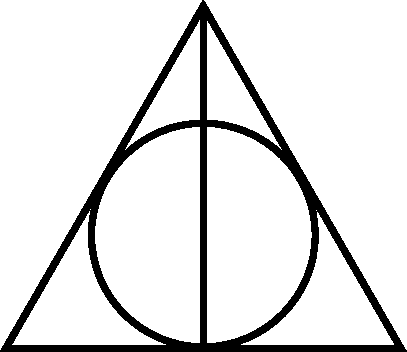
\includegraphics[scale=0.125]{images/Deathly_Hallows_Sign.png}
\end{center}
}
\vspace*{\fill}
\clearpage

%  LocalWords:  nd Kahneman eeeeviiil medi Hmmm stalkery
